\section{Application: App/OS Behavior}
\label{sec:characterize-app}
In this section we describe how we use \meddle to identify privacy leaks and tracking by third parties 
in mobile systems. While previous work identifies many of the same issues, they lack a general 
way to identify leaks using network flows alone, and they provide no portable way to block those 
activities. In the following sections, we describe how we identify the apps responsible for privacy 
leaks and tracking, regardless of whether they use SSL. Then we describe a system that visualizes 
this activity and allows users to block it.

\subsection{Mapping Network Flows to Apps}
\section{Traffic Classification}
\label{sec:classification-methodology}

In this section, we revisit mobile traffic characterization and classification, using a comprehensive 
view of Internet traffic from mobile devices. Previous work uses passively gathered data 
to characterize such traffic, which can be useful for a variety of important topics that include 
traffic engineering, optimization of network-enabled apps and understanding threats to user privacy. 
The following sections show that  previous approaches to classifying traffic fail to identify
apps responsible for that traffic most of the time and that \platname{} facilitates a first look at 
determining which apps generate traffic over SSL connections.

% 1) for the users in our study, traffic over WiFi and cellular networks 
%are qualitatively different, and studies that focus on only one technology will miss approximately 
%half of the traffic generated by devices; 

\subsection{Classification of Mobile Apps and Services}

Our \mobWild dataset suggests that apps, OS services and libraries often rely on HTTP and SSL to exchange data~\cite{maier:mobtraffic,falaki:mobileusage,xu:appusage}.
%To analyze the behavior of mobile services we need to first associate the observed flows with the applications and the OS services responsible for the flows.
In the following analysis, we focus on identifying the apps, OS services, and other services responsible for these HTTP and SSL flows. 
We use ground-truth data from controlled experiments to show that the previous approach for classification fails 
for most popular apps; we then develop techniques to improve this mapping and apply it to our \mobWild dataset. 

\subsubsection{HTTP Traffic Classification}

Mapping network flows to apps is an important step for determining the origins of potentially costly 
network traffic, and for identifying which apps are responsible for privacy leaks. One approach for this is to use the \useragent field on app-generated traffic.
Previous work uses this to classify traffic, but only at the granularity of the app category~\cite{erman2011http,xu:appusage,maier:mobtraffic}. 
Below we describe the limitations of this approach for a large fraction of apps, and how we improve classification using only header information (\ie HTTP and lower layers). 
%use the results from our controlled experiments and the \mobWild dataset to argue that the \useragent can be used to identify flow from popular iOS and Android applications, for flows that do not contain a useful \useragent we fall back to classifying identifying the web-service using the \httphost field.

To motivate why this is a difficult problem, consider the following scenario. When using the \httphost field in the HTTP header, a flow with \emph{static.ak.fbcdn.net} in the \httphost field implies that it contacted one of the Facebook servers; however, the \httphost field does not tell us whether Facebook is accessed via a Web browser or through the native Facebook app. Similarly, the \useragent field can specify an app name, but it is not required to do so. Below, we show the effectiveness of combining these approaches. 


%\begin{table} 
%    \begin{small}
%    \begin{tabular}{|p{0.1\columnwidth}|p{0.18\columnwidth}|p{0.1\columnwidth}|p{0.13\columnwidth}|p{0.17\columnwidth}|}
%       \hline
%       {\bf OS}& {\bf Store} &{\bf \# Apps}&{\bf Generated HTTP}& {\bf Correct User-Agent} \tabularnewline
%       \hline    
%       iOS     & App Store   & 209 & 176 & 149 (84.6\%) \tabularnewline
%       Android & Google Play & 100 & 92  & 21 (22.8\%)  \tabularnewline
%       Android & Third party & 908 & 494 & 32 (6.4\%)   \tabularnewline
%       \hline
%    \end{tabular}
%    \end{small}
%    \caption{Classification of applications based on \useragent. \emph{We observe that we were table to classify \tbd{} of iOS and \tbd{} of Android applications that generated traffic during our experiments.}}
%    \label{tab:classification-success}
%\end{table}


\begin{table} 
     \centering
     \begin{small}
     \begin{tabular}{|p{0.05\columnwidth}|p{0.08\columnwidth}|p{0.07\columnwidth}|p{0.08\columnwidth}|p{0.09\columnwidth}|p{0.09\columnwidth}|p{0.09\columnwidth}|p{0.09\columnwidth}|}
        \hline
        {\bf OS}&{\bf Store}&{\bf Apps}&{\bf Gen.}&\multicolumn{2}{|c|}{\bf Host} & {\bf User-}&{\bf Combi-} \tabularnewline
        \cline{5-6}    
             &        &     & {\bf HTTP} & {\bf App. } & {\bf Org.}& \bf{Agent}   & \bf{nation}  \tabularnewline                
        \hline    
        iOS  & Apple  & 209 & 176 & 83 (47.1\%)  &  119 (67.6\%)   &  149 (84.6\%)& 157 (89.2\%) \tabularnewline
        \hline
        And. & Google & 100 & 92  & 41 (44.5\%)  &  54 (58.6\%)    &  21 (22.8\%) &  59 (64.1\%)  \tabularnewline
        \hline    
        And. & Other  & 908 & 494 & 106 (21.4\%) & 139 (28.1\%)     &  32 (6.4\%)  &  163 (32.9\%)  \tabularnewline
        \hline
     \end{tabular}
     \end{small}
     \caption{Classification of apps based on \httphost and \useragent. \emph{A large majority of iOS apps use dedicated \useragent strings to fetch data over HTTP. A combination of \useragent and \httphost can be used to identify the majority of Android and iOS apps.} }
     \label{tab:classification-success}
\end{table}

%%
%% No HTTP Traffic from 209 - 38 = 171; 171 + 5 (OS possibly - confirm) = 176  ,
%% 181 unique signature, 7*2 = 14 duplicate (fooducate, fdct). 
%% 174 unique application signatures found
%% 5 UA belonged to OS services, geoservices, applecoremedia, gamekit, securityd, mmsdk 
%% Ads from 98 - 4 -> 94 labels
%% Rough estimate of HTTP for apps because mapping  -- 414 files without HTTP
%%%

\noindent\textbf{Controlled experiments.}
In Table~\ref{tab:classification-success} we present results from our classification study using controlled experiments. To 
the best of our knowledge, we are the first to attempt to use ground-truth information to evaluate the 
effectiveness of app classification using only header data.
 

\emph{iOS:}
First, we note that 176 of the 209 iOS apps we manually tested generated HTTP traffic.
We observe that the \httphost field uniquely identified the corresponding app for 47\% of the iOS apps we tested (column 5).
%; the flows containing the application signature was responsible from 15\% to 98\% of the traffic volume from the application. 
%\tbd{TODO: This was done only for a sample of applications -- I shall perform this test in detail after deadline}
The \httphost field also can identify the provider that released an app.
For example Zynga offers multiple games with dedicated apps that contact Zynga properties.
When classifying apps according to their provider, we observe in Table~\ref{tab:classification-success} (column 6) that our classification success increases to 67\% of iOS apps. 


\emph{Android:} We observe similar results for flows from apps released through Google Play.
However, for the apps from the Third-party store we observe that the \httphost field is less effective. 
Primarily this is due to the fact that a majority of the apps we tested (about 77\%) were stand-alone services such as games where the provider did not use its own Web service. Instead, these apps either contacted some advertisement sites or sites hosted by CDNs. 
While we can use the \httphost field to identify these 3rd-party sites contacted by an app, we cannot determine which app generated the traffic. 

\begin{table}
\begin{small}
\begin{tabular}{|l|p{0.85\columnwidth}|}
\hline
{\bf No. } & {\bf User-Agent}\tabularnewline
\hline
1 & YahooMobileMail/1.0 (Android Mail; 1.4.6) (crespo;samsung;Nexus S;4.1.2/JZO54K)\tabularnewline
\hline
2 & AppleCoreMedia/1.0.0.10A523 (iPad; U; CPU OS 6\_0\_1 like Mac OS X; en\_us) \tabularnewline
\hline
3 & Dalvik/1.6.0 (Linux; U; Android 4.2.2; Nexus 4 Build/JDQ39) \tabularnewline
\hline
\end{tabular}
\end{small}
\caption{Sample \useragent strings. \emph{The first string contains the app identifier, the second hides the app and describes the OS service/library used, while the third does not contain any useful signature.}}
\label{tab:user-agent}
\end{table}

\emph{Augmenting with \useragent: } We now show that by augmenting the information in the \useragent to the information gained by the \httphost field, we can classify a majority of iOS and Android apps. 
In our controlled experiments we observed a non-empty \useragent string in more than 99.7\% of the HTTP flows from iOS and 90.9\%flows from Android. 

A \useragent string may contain an app identifier and other auxiliary information such as details of the OS, manufacturer, and compatibility with Web browsers~\cite{mozilla:useragentdetection}. 
For example, the first \useragent in Table~\ref{tab:user-agent} contains the information of the app, YahooMobileMail, while the second \useragent hides the app and specifies the \emph{AppleCoreMedia} service of iOS, and the third does not provide any useful information. 
To extract the app information, we use a set of regular expressions to filter out the auxiliary information in the \useragent and further cluster these extracted tokens using the edit distance between the tokens.\footnote{We plan to release this code along with \platname package.}

In Table~\ref{tab:classification-success} we observe that 176 of the 209 iOS apps generated HTTP traffic, 149 of these were correctly identified based on the signatures in their \useragent, which we verified by manual inspection.
In contrast, our \useragent based identification was able to correctly identify less than 23\% of the Android apps that generated HTTP traffic. 
For the 27 iOS apps which we failed to identify, we observed signatures for OS services and libraries, such as \emph{Apple Core Media}, \emph{Game Kit}, \emph{Geo Services}, etc. and signatures of third-party libraries and services such as \emph{Google Analytics} and \emph{Adobe Air}.
Similarly, the majority of Android HTTP traffic contained flows with the default \useragent (similar to the third \useragent in Table~\ref{tab:user-agent}).
Further, for the apps from the third-party store, we observe that the \useragent for ads and analytics libraries such as \emph{Google Analytics} and \emph{Adsense for Mobile} were the most common \useragent after the default \useragent.

To wrap up, \useragent is more effective for classifying iOS apps and \httphost is more effective for Android apps; however, neither alone is a complete 
solution. A topic of future work is to explore packet contents using deep packet inspection -- it is likely that apps are identifying themselves to CDNs and 
ad/analytics servers in the payload. 

\begin{figure}
\subfloat[iOS]{\label{fig:http-wordcloud-ios}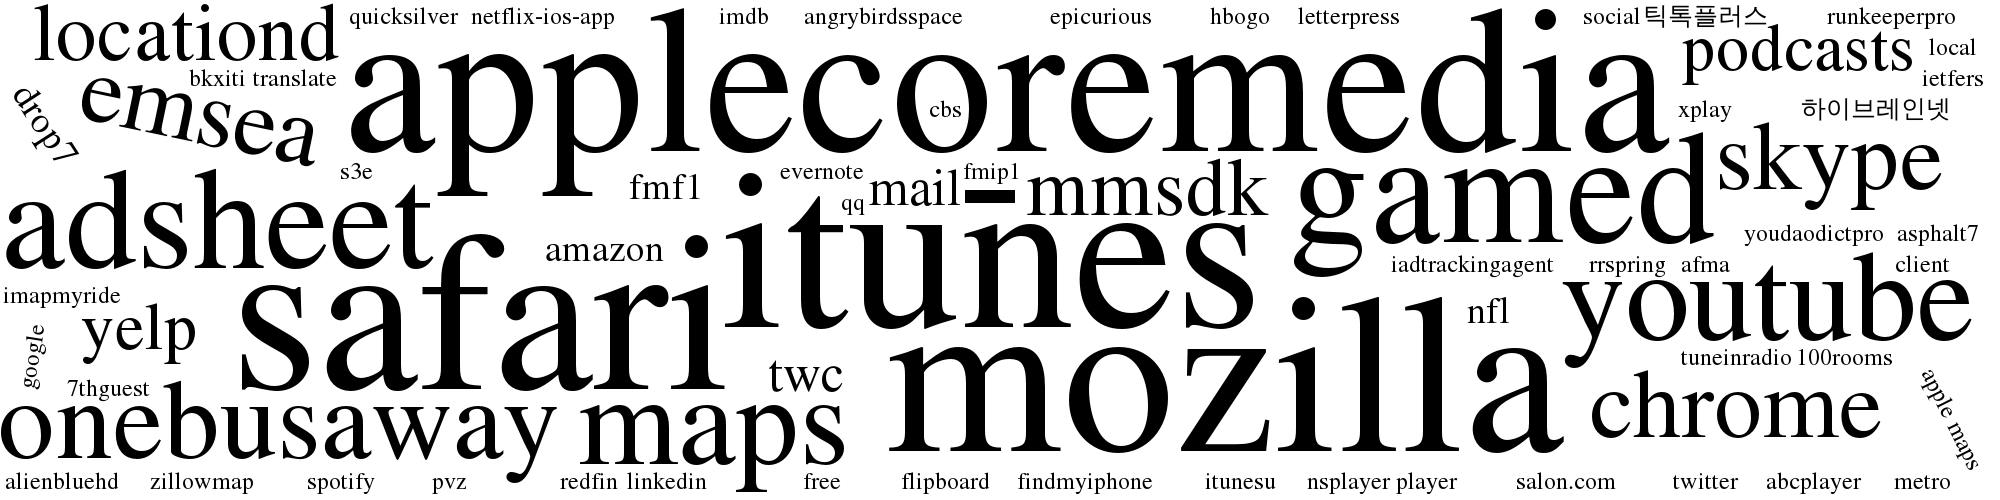
\includegraphics[width=\columnwidth]{figures/wordcloud_useragentsignature_ios_image.png}}\newline
\subfloat[Android]{\label{fig:http-wordcloud-android}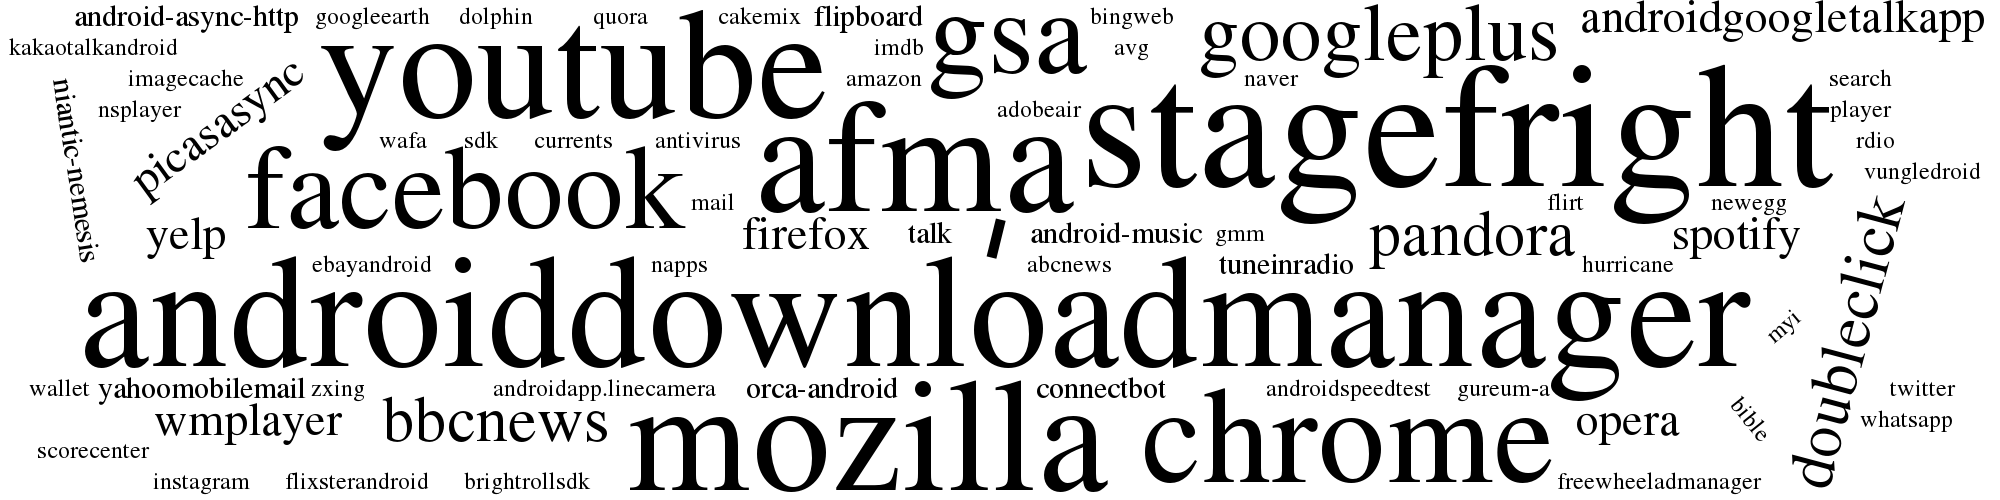
\includegraphics[width=\columnwidth]{figures/wordcloud_useragentsignature_android_image.png}}
\caption{\useragent signatures in  iOS and Android HTTP flows. \emph{The font weight represents the number of users for which a particular signature was observed.}}
\vspace{\postfigspace}
\label{fig:http-wordcloud}
\end{figure}

\textbf{In the wild data.}
We now describe the results of our classification on data gathered from our user study.
Using only the \useragent on the \mobWild dataset we were able to map flows to 243 iOS and 84 Android apps, OS libraries, and services. 
The \emph{word cloud} in Figure \ref{fig:http-wordcloud} contains the summary of our results; the font size of a signature is proportional to the number of users for which the signature was observed.
Along with signatures of apps such as iTunes and YouTube, we also observe signatures of the \emph{Apple Core Media} and \emph{Stagefright} services that are responsible for downloading media content on iOS and Android devices respectively.
%Across the iOS and Android devices, we observe a total of \tbd{1435} unique \useragent strings that produce \tbd{361} unique signatures which we cluster to \tbd{} different apps and services. 
For the iOS devices in the \mobWild dataset, we observe a signature of \emph{Apple Core Media} in more than 98.45\% of the content downloaded from the YouTube servers.
Similarly, depending the Android version we observe either the signature for Stagefright or no app or OS service signature for YouTube traffic to Android devices depending on the OS version. 
We observe a similar signatures for other popular media services such as Netflix, YouTube, Vimeo, Pandora, etc.
Because we cannot identify the app used to access these services, we fall back to the \httphost field to identify these Web services.

\begin{table}
\centering
\begin{small}
\begin{tabular}{|p{0.25\columnwidth}|c|c|c|c|}
\hline
\multirow{2}{*}{\bf Category} & \multicolumn{2}{c|}{\bf \% of iOS Traffic } &  \multicolumn{2}{c|}{\bf \% of Android Traffic } \tabularnewline
\cline{2-5}
  & {\bf Bytes}  & {\bf Flows} & {\bf Bytes} & {\bf Flows}   \tabularnewline
\hline
Media (Popular)         & 51.405  & 12.131 & 65.922 & 22.377 \tabularnewline
\hline
Application             & 33.987  & 80.758 & 31.353 & 77.498 \tabularnewline
\hline
Media (Other)           & 14.572  &  5.914 &  2.712 &  0.044 \tabularnewline
\hline
Other                   &  0.036  & 1.1963 &  0.013 &  0.081 \tabularnewline
\hline
{\em total}             & 100 (\%)& 100 (\%)& 100 (\%) & 100 (\%) \tabularnewline
\hline
\end{tabular}
\end{small}
\caption{Classification of HTTP Traffic. \emph{While popular media services such as Netflix and YouTube dominated the traffic volume, the applications were responsible for more than 80\% of iOS and 77\% of Android HTTP flows.}}
\label{tab:classify-http}
\vspace{\postfigspace}
\end{table}

In Table~\ref{tab:classify-http}, we observe that with a combination of \useragent and \httphost field in HTTP headers, we were able to classify more than 98\% of the traffic in terms of flows and bytes from iOS and Android devices.
We observe that media from popular hosts in our \mobWild dataset, including Netflix, YouTube, Pandora, Spotify, and Vimeo, contribute to more than 50\% of the traffic volume from iOS and Android devices.
Similarly, we observe that apps identified based on the \useragent  were responsible for more than 77\% of flows from Android and iOS devices. 
We also observe that media (identified based on the signatures such as \emph{Apple Core Media} and \emph{Stagefright}) served from CDNs and others hosts from which we could not identify the Web service from other fields in the HTTP header, and also the DNS responses before the HTTP flows, comprises 14.5\% of the traffic volume for the iOS devices in our dataset.

\subsubsection{Classification of SSL Traffic.}

Unlike HTTP flows, SSL flows provide limited information in plaintext that can be used to identify the apps. 
For the traces captured during our controlled experiments, we were able to observe HTTP requests and responses 
after decrypting with SSL bumping. We can classify such flows using the techniques described in the previous section. 
However, we did not perform SSL bumping for the devices in the \mobWild dataset, so we now describe how to 
classify SSL flows \emph{without decryption}. As we show below, we used the port number, the SSL certificate with server 
name identification, and DNS queries to identify the source of SSL traffic. 

% \begin{table}
% \centering
% \begin{small}
% \begin{tabular}{|p{0.25\columnwidth}|c|c|c|c|}
% \hline
% \multirow{2}{*}{\bf Service} & \multicolumn{2}{c|}{\bf iOS} &  \multicolumn{2}{c|}{\bf Android} \tabularnewline
% \cline{2-5}
%   & {\bf Bytes}  & {\bf Flows} & {\bf Bytes} & {\bf Flows} \tabularnewline
% \hline
% HTTPS                   & 91.287 & 81.960 & 97.852 & 97.168    \tabularnewline
% \hline
% Mail                    &  6.700 & 15.872 & 0.689  & 0.320  \tabularnewline
% \hline
% Notification            &  1.412 & 1.553  & 1.321  & 2.100  \tabularnewline
% \hline
% Other                   &  0.601 & 0.615  & 0.138  & 0.412 \tabularnewline
% \hline
% {\em total}             & 100 & 100 & 100 & 100 \tabularnewline
% \hline
% \end{tabular}
% \end{small}
% \caption{Classification of SSL Traffic based on port number. \emph{HTTPS is the most popular service that uses SSL in the \mobWild dataset.}}
% \label{tab:classify-ssl-port}
% \end{table}

Mobile devices use SSL for various services including mail, notifications, instant messaging, and Web browsing.
Services such as mail, instant messaging, and notifications are documented to use dedicated port numbers of their traffic.
%\footnote{We also use the AS for identifying push notification messages as detailed in \fref{sec:characterize-os}.}
On using port numbers, we observe in that more than 99\% of the SSL flows observed in our controlled experiments were due to HTTPS, the rest of the flows were due to email, instant messaging, and OS notification services. 
We therefore focus our attention on identifying the Web services responsible for the HTTPS flows. 

%\tbd{THE NUMBERS FOR THIS ARE FROM THE WILD MEASUREMENTS. ON SIMPLE GLANCING I WAS ABLE TO OBSERVE SIMILAR NUMBERS. I SHALL ADD THEM BY THE TIME OF THE CAMERA READY}

\noindent\textbf{Classification techniques.} We first use the common name (CN) field of certificates to identify the servers that exchanged data using HTTPS.
We observe that less than 25\% of the HTTPS traffic from iOS and Android contains the fully qualified domain name (FQDN) in the subject of the certificate; the rest of the traffic either contains regular expressions such as *.google.com in the certificate.
% or is a continuation of a previous SSL session. 
To further resolve the hostnames, we rely on \emph{server name indication} used by SSL flows~\cite{rfc:servernametls}.
Servers that host multiple services use the \emph{server name indication} to distinguish these services.   
For example, we observe a \emph{server name indication} of \emph{plus.google.com} and \emph{s.youtube.com} in two flows that used a certificate with a CN \emph{*.google.com}.
However, we observe that by using either the certificate or the \emph{server name} we were able to identify the name of the Web service in less than 40\% of iOS and Android HTTPS traffic.

\noindent\textbf{DNS mapping.} For the remaining flows we use DNS requests made by the mobile devices before starting the HTTPS flows, a technique similar to DN-Hunter~\cite{bermudez:dnhunter}.
DN-Hunter relies on the most recent FQDN that corresponds to the IP address, however in our controlled experiments we observe Android and iOS devices use the first entry in DNS response while resolving \emph{hostnames}.
We therefore use the latest DNS response that contains the IP address of the Web service in the first position of the DNS response. 
%FOR THE WILD: Indeed, for 97.8\% of the Android and 83.4\% of the iOS HTTPS traffic that we could not classify using other fields, we observe that the latest DNS response before the flow started contained the IP address of the webservice as the first entry in the DNS response\footnote{The share of SSL traffic where the latest DNS response contains the IP address of the web-service in the first position is 97.4\% for Android and 88.6\% of iOS}. 
Indeed, for more than 99\% of the iOS and Android HTTPS traffic that we could not classify using other fields, we observe that the latest DNS response before the flow started contained the IP address of the Web service as the first entry in the DNS response.
Despite the potential usefulness of DNS responses, we give a high priority to the server-name and the certificates because we observed that for flows that contained the server name did not contain the same name in the DNS response for 9.2\% of the iOS traffic and 5.6\% of Android traffic.

\begin{table}
\centering
\begin{small}
\begin{tabular}{|c|c|}
\hline
{\bf iOS} & {\bf Android} \tabularnewline
\hline
imap.gmail.com & picasaweb.google.com \tabularnewline
www.google.com & www.googleapis.com \tabularnewline
sphotos-a.xx.fbcdn.net & android.clients.google.com \tabularnewline
itunes.apple.com  & clients4.google.com \tabularnewline
m.google.com & fbcdn-photos-a.akamaihd.net \tabularnewline
\hline
\end{tabular}
\end{small}
\caption{Popular hostnames in observed in SSL flows from iOS and Android based on traffic volume. \emph{Hostnames such as www.googleapis.com hide the underlying app and Web service.}}
\label{tab:sslclassify-popular-host}
\end{table}

\noindent\textbf{Classification results.} In Table~\ref{tab:sslclassify-popular-host} we present the top five hostnames according to traffic volume -- responsible for 66\% of iOS and 54\% of Android traffic by volume in the \mobWild dataset. 
We observe that even when a hostname is specified we cannot uniquely uniquely identify the Web service for some flows.
For example, \emph{www.google-apis.com} and \emph{clients4.google.com} offer limited information on the app or Web service that is responsible for the content; at best we can infer these flows belong to some Google service.
In contrast, the  hostname \emph{fbcdn-photos-a.akamaihd.net} is a strong indication that the traffic is due to Facebook (due to ``fbcdn'').

\begin{table}
\centering
\begin{small}
\begin{tabular}{|p{0.35\columnwidth}|c|c|c|c|}
\hline
\multirow{2}{*}{\bf Service} & \multicolumn{2}{c|}{\bf \% of iOS Traffic} &  \multicolumn{2}{c|}{\bf \% of Android Traffic} \tabularnewline
\cline{2-5}
  & {\bf Bytes}  & {\bf Flows} & {\bf Bytes} & {\bf Flows} \tabularnewline
\hline
Mail                 & 9.970    & 62.168   & 1.626  & 1.565 \tabularnewline
\hline
Social Networking    & 12.491   & 6.683    & 36.661 & 22.352 \tabularnewline
\hline
App Store   & 5.457    & 3.463    & 0.044  & 0.036 \tabularnewline
\hline
Instant Messages     & 0.982    & 7.089    & 1.411  & 3.109 \tabularnewline
\hline
Other Google Services & 58.665   & 13.32510 & 45.024 & 46.089 \tabularnewline
\hline
\emph{total (\%)}         & 87.564   & 92.728   & 84.776 & 73.151 \tabularnewline
\hline
\end{tabular} 
\end{small}
\caption{Classification of \mobWild SSL traffic based on names in certificate, server name identification, and DNS request.}
\label{tab:classify-ssl-traffic}
\end{table}

In Table~\ref{tab:classify-ssl-traffic} we present our SSL classification results.
We observe that the iOS devices in our dataset generated a significant number of e-mail flows.
Similarly, we were able to group 12.5\% of iOS and 36.7\% of Android traffic with social network services that includes \emph{Google Plus, Facebook, and Twitter}.
We speculate the increase in traffic share for Android devices is because Android devices offer services to backup photos on \emph{Google Plus}.
Similarly, we observe that 5.4\% of the traffic from iOS devices was from Apple stores while we observe only 0.04\% of traffic to the \emph{Google Play} store. 
This low share is because Google can use hosts matching the pattern \emph{client*.google.com} to serve different Web services.
We observed a similar behavior in our controlled experiments, and we group such traffic as \emph{other Google services}.
Indeed, in Table~\ref{tab:classify-ssl-traffic} we observe that Google is the largest target of SSL traffic for iOS and Android devices in our dataset. 
The next most popular target for SSL traffic is social networking sites.

Having developed techniques to map network flows to apps, we use this classification to study the apps responsible for 
leaking private information.

% Popular webservices such as google are known to use the same pool of IP addresses for various applications, for example the IP for gmail may also be used for search. 
% In \fref{fig:ssl-classification-app-service} we present the fraction of SSL traffic where the most recent DNS response contained the IP address of the SSL flow in the first position. 
% We observe that for the majority of SSL traffic by volume and flows can be classified by using the DNS responses. 

% \begin{table}
% \centering
% \begin{small}
% \begin{tabular}{|p{0.35\columnwidth}|c|c|c|c|}
% \hline
% \multirow{2}{*}{\bf Service} & \multicolumn{2}{c|}{\bf iOS} &  \multicolumn{2}{c|}{\bf Android} \tabularnewline
% \cline{2-5}
%   & {\bf Bytes}  & {\bf Flows} & {\bf Bytes} & {\bf Flows} \tabularnewline
% \hline
% FQDN in Certificate    & 24.274 & 31.423  & 19.318 & 29.424 \tabularnewline
% \hline
% Regular expression     & 50.463 & 35.318  & 42.427 & 31.670 \tabularnewline
% \hline
% No Subject or CN       & 25.263 & 33.259  & 38.254 & 38.906 \tabularnewline
% \hline
% {\em total}            & 100 & 100 & 100 & 100 \tabularnewline
% \hline
% \end{tabular}
% \end{small}
% \caption{Classification of HTTPs based on certificates.}
% \label{tab:classify-http-cert}
% \end{table}

% We observe that more than 98\% of HTTP traffic from Android and iOS devices in the \mobWild dataset have a valid \useragent string; we observe a total of 1435 unique \useragent strings across Android and iOS devices. 
% These \useragent strings contain an application identifier and other auxiliary information such as details of the OS, manufacturer, display resolutions, carrier, and information such as versions and compatibility with other browser engines~\cite{mozilla:useragentdetection}. 
% We use regular expression to extract the tokens that contain the application information, and cluster these tokens using edit distance\footnote{We plan to release this code along with \platname package.}.
% At the end of this process we were able to identify 361 unique signatures which we resolve as either applications or OS services. 

% In \fref{fig:http-wordcloud} we present a \emph{word cloud} of the signatures we were able to extract from \useragent field; the text size of the signature represents the number of users for which the signature was observed.
% Despite the usefulness of the \useragent, we observe that relying only on the \useragent is not sufficient to identify the application.
% For example, we observe the signatures \emph{applecoremedia} and \emph{stagefright} in the \emph{word cloud} for iOS devices and Android devices, signatures of the OS services responsible to download media content.

% The iOS devices rely on AppleCoreMedia service~\cite{apple:coremedia} to download media content.
% We therefore observed the signature of AppleCoreMedia in more than 98.45\% of the content downloaded from the YouTube servers (which we identify based on the \httphost field in the \httpget requests). 
% Similarly, depending the Android version we observe either the signature for Stagefright\cite{android:stagefright} or no application or OS service signature for YouTube traffic to Android devices. 
% Indeed, we observed signatures for popular media services such as Netflix, YouTube, Vimeo, Pandora, etc. in the \httphost field in the majority traffic from iOS devices and Android devices. 
% We therefore used the \httphost field to classify media content.



\subsection{Identifying Privacy Leaks}
Privacy has rapidly become a critical issue for networked services, as large numbers of organizations develop 
extensive tracking infrastructure to gather information from users for ads and analytics. While the problem 
is well known and has been extensively studied in previous work~\cite{roesner:webtrackers,leontiadis:mobileads,vallina-rod:ads}, in this section we explore the potential to 
identify personals identifiable information (PII) exclusively from passively gathered app traces. Our key 
contributions are 1) we conduct controlled experiments to identify how PII is being leaked by apps via 
their network flows and 2) use SSL bumping enabled by \platname{} to understand how this information is being shared over 
secure channels (in addition to those revealed in the clear). 
For our analysis we focus on {\it what} PII is sent,  {\it to whom} is the PII sent, and {\it how frequently} is PII sent.
%To answer these questions, we rely on the controlled experiments and the \mobWild dataset.

We evaluate PII in terms of two threat models. First, we assume a passive eavesdropper that can sniff 
traffic over open WiFi APs or within a cellular provider. Any PII sent unencrypted is available to the attacker. 
Second, we assume an attack conducted by (or on) a third-party service that is able to identify a user's fine-grained locations 
over time. 

\begin{table*}[t]    
    \centering
    \begin{small}
    \begin{tabular}{|l|l|l|l|l|l|l|l|l|l|}
       \hline
       {\bf Store}&{\bf Platform}&{\bf \# Apps}&{\bf Email}& {\bf Location}& {\bf Name} &{\bf Password}& {\bf Device ID}& {\bf Contacts}& {\bf IMEI}\\
       \hline
       App Store&iPhone&209&13 (6.2\%) &20 (9.5\%)&4 (1.9\%)&6 (2.87\%)&4 (1.9\%)&0 (0\%)&0 (0\%)\\
       \hline
       Google Play&Android&100&3 (3\%)&10 (10\%)&2 (2\%)&1 (1\%)&21 (21\%)&0 (0\%)&13 (13\%)\\
       \hline
       Third Party&Android&908&1 (0.1\%)&32 (3.5\%)&2 (0.2\%)&0 (0\%)&95 (10.4\%)&4 (0.4\%)&48 (5.3\%)\\
       \hline
    \end{tabular}
    \end{small}
    \caption{Summary of personally identifiable information leaked in plaintext (HTTP) by Android and iPhone apps. \emph{The popular iOS apps tend to leak the location information in the clear while Android apps leak the IMEI number and Android ID in the clear. \tbd{Nice if we had same number in Google Play and App Store.}}}
    \label{tab:pii}
\end{table*}

\subsection{Controlled experiments}

For our experiments, we created fake user accounts with fake contact
information, and fake Twitter and Facebook accounts.  Our goal is to
detect if any PII---email
address, phone number, IMEI number---stored on the device is leaked
across the network over HTTP or HTTPS (using the SSL bumping plugin).
Some of this information is required for normal app operation; however, we strongly believe that such information should
never travel across the network in plaintext (HTTP). 

In Table~\ref{tab:pii}, we present the different PII leaked by both Android and iPhone apps.  We observe that
the IMEI, a unique identifier tied to a phone, is the most commonly
leaked PII by Android apps.  This IMEI can be used to track
and correlate a user's behavior across Web services.  Similarly, we
observe that Android apps leak the Android ID, a unique
identifier tied to an Android device.  In Table~\ref{tab:pii}, we also
observe that other information like contacts, emails, and passwords
are leaked in the clear.  The email address, the address used to sign
up for the services, was leaked in the clear by 13 iOS and 3 Android
apps from our set of popular apps.

While only one Android app (belonging to the \emph{Photography} category) leaked a password in the clear, 
we were surprised to learn that six of the most popular iOS apps send user 
credentials in the clear, \emph{including the password}. Particularly disconcerting 
is our observation that an app in the Medicine category -- which the provider claims has ``\emph{1 million active members 
of which 50\% are US physicians}'' -- sends the user's first name, last name, 
email, password, and zip code in the clear. Given US physician access to highly sensitive 
data like medical records, we believe it is particularly important for this app to protect 
user credentials (which are often used for multiple services). 

% For your eyes only ;)
%services.epocrates.com  Mozilla/5.0 (iPhone; U; CPU iPhone OS 4_0 like Mac OS X; en-us) AppleWebKit/532.9 (KHTML, like Gecko) Version/4.0.5 Mobile/8A293 Safari/6531.22.7   1370172894.1735 JXMXaFcr2Pd 10.11.4.52  55904   63.241.66.139   80  7   GET /userprofile/userprofile/userprofile/userprofile?datatype=json&os=6.1.3&device_model=iPhone&appVersion=5.2&appId=nc-2&data={"countryId":"10","lastName":"Test","firstName":"Meddle","password":"epocratespwdW1","passwordConfirm":"epocratespwdW1","email":"mailmeddle@yahoo.com","occupationId":"56","zipCode":"98105"}&action=useraccount&platform=14&subaction=createuser    -   0   40001   200 OK  -   -   -   (empty) -   -   -   text/plain  -   -   -   0       -   -   shen

\begin{table}
    \centering
    \begin{small}
    \begin{tabular}{|l|c|c||c|}
       \hline
       {\bf Host}&{\bf IMEI}&{\bf Device ID} & {\em Ads \& Analytics} \tabularnewline
       \hline              
       chartboost.com                & \checkmark & \checkmark & \checkmark  \tabularnewline
       tapjoyads.com                 & \checkmark & -          & \checkmark  \tabularnewline
       getjar.com                    & \checkmark & \checkmark & -   \tabularnewline
       pocketchange.com              & \checkmark & \checkmark & -   \tabularnewline
       iheart.com                    & \checkmark & \checkmark & -   \tabularnewline
       aarki.net                     & \checkmark & -          & \checkmark  \tabularnewline
       zynga.com                     & \checkmark & -          & -   \tabularnewline
       droidsecurity.appspot.com     & \checkmark & -          & -   \tabularnewline
       google.com                    & -          & \checkmark & -   \tabularnewline
       flurry.com                    & -          & \checkmark & \checkmark  \tabularnewline
       groupon.com                   & -          & \checkmark & -   \tabularnewline
       \hline
    \end{tabular}
    \end{small}
    \caption{Top 10 hosts that receive the IMEI or Device ID over HTTPS. \emph{Hosts are ordered by the number of flows that send the IMEI number, followed by the number of flows that send the device ID over HTTPS. Four of the top 10 hosts that receive this information are ads and analytics sites.}}
    \label{tab:pii-leakage-https-sites}
    \vspace{\postfigspace}
\end{table}

During our experiments, we observed that PII is also sent over HTTPS.  In the following, we
focus on device identifiers such as the IMEI and the Android device
ID.  In Table~\ref{tab:pii-leakage-https-sites}, we present the top 10
sites ordered by the number of flows that sent the IMEI over HTTPS.  We
observe that four of the top 10 sites that receive this information
are ads and analytics (A\&A) sites.

Our observations highlight the limitations of current mobile OSes with 
respect to controlling access to PII via app permissions. In particular, it is unlikely that users are 
made aware that they are granting access to PII for A\&A sites when embedded 
in an app that serves a different purpose. This problem is pervasive: of the 77 sites
that received either the IMEI or Device ID in the clear or over HTTPS,
35 sites were third party ads and analytics sites.

We note that our observations are a conservative estimate of PII leakage. Specifically, 
we cannot detect PII leakage if the data is obfuscated (\eg via hashing). Regardless, 
our study showed that a significant amount of PII leaks not only through unobfuscated 
channels but even unencrypted ones. 

%In summary, we use our controlled experiments to identify PII leaks on
%both HTTP and HTTPS, and we show that PII are leaked to third party
%sites such as ads and analytics. These controlled experiments are a
%practical use case of \platname, experiments requiring warranty
%voiding the devices otherwise. In particular, \platname{} enable to
%reveal PII leaks over HTTPS.
%However, we would like to point out that we were not able to analyze traffic in which the data sent was encoded and exchanged as binary objects. 

%Stats value 13 of 22 in the clear device ID, 16 of 39 IMEI clear,  3 of 6 IMEI HTTPs, 3 of 10 device HTTPs}

\subsection{PII in the Wild}

In the previous section, we focused on controlled experiments. We now
analyze the \mobWild{} dataset. We do not use SSL bumping on this data 
for privacy reasons. Instead, we focus on information is leaked in the clear.

\begin{figure}[tb]
\subfloat[Apps leaking location in the clear.]{\label{fig:location-cloud} 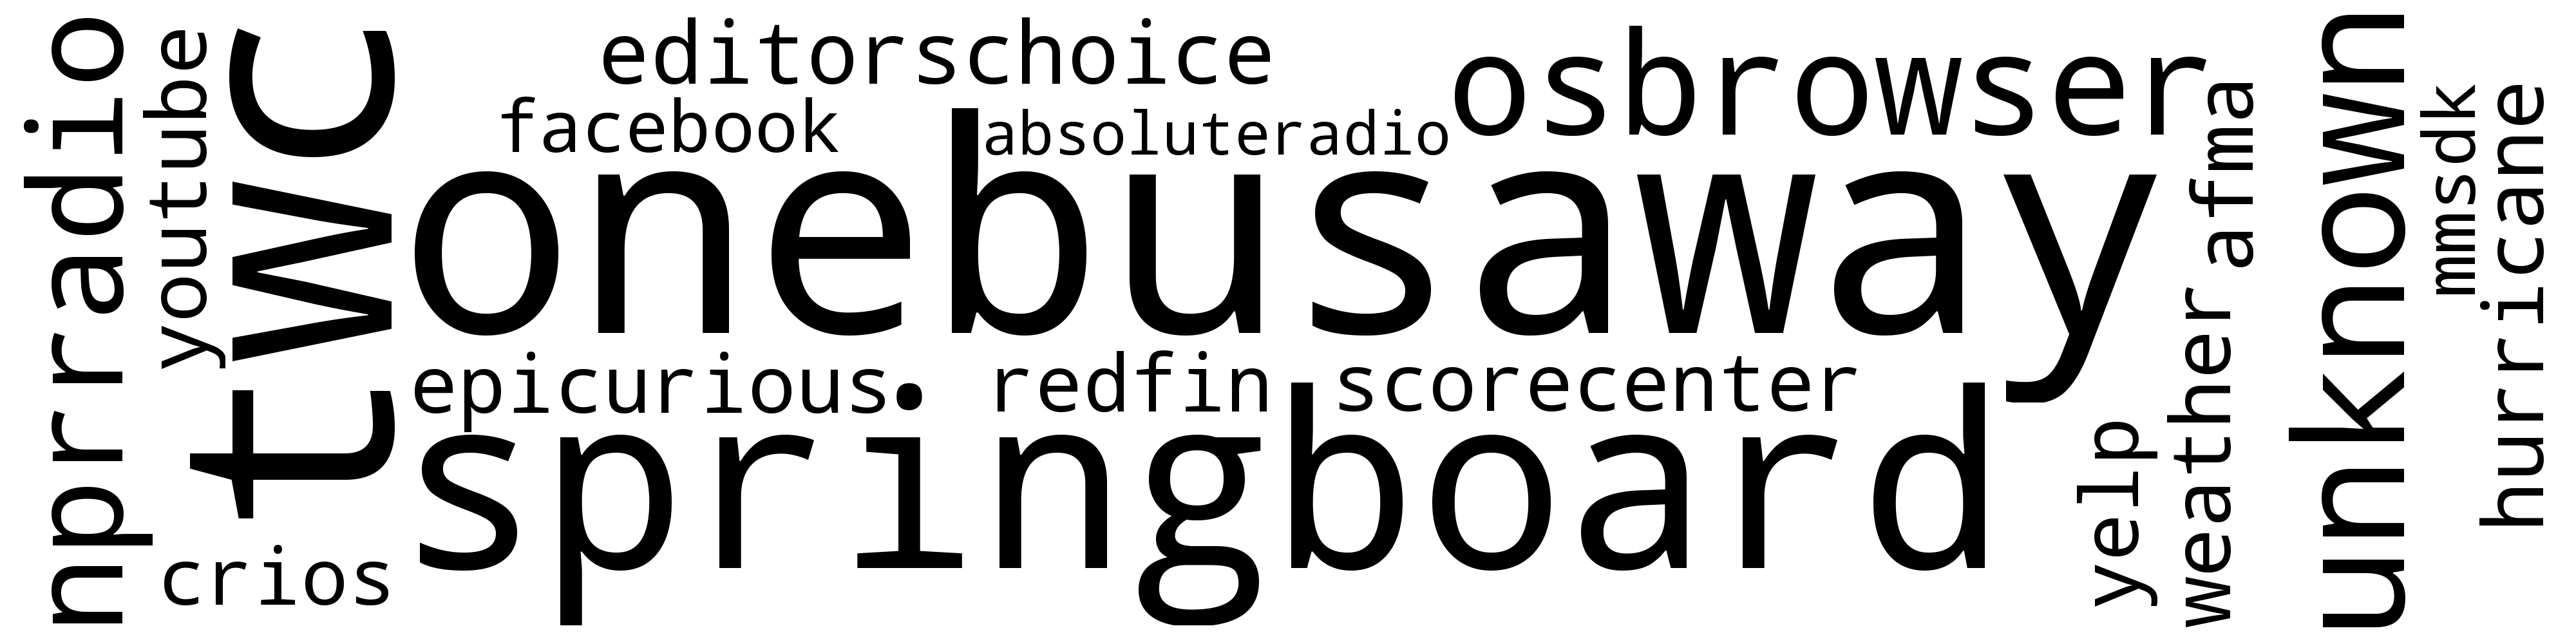
\includegraphics[width=\columnwidth]{figures/wordcloud_useragentsignature_location_image.png}}
%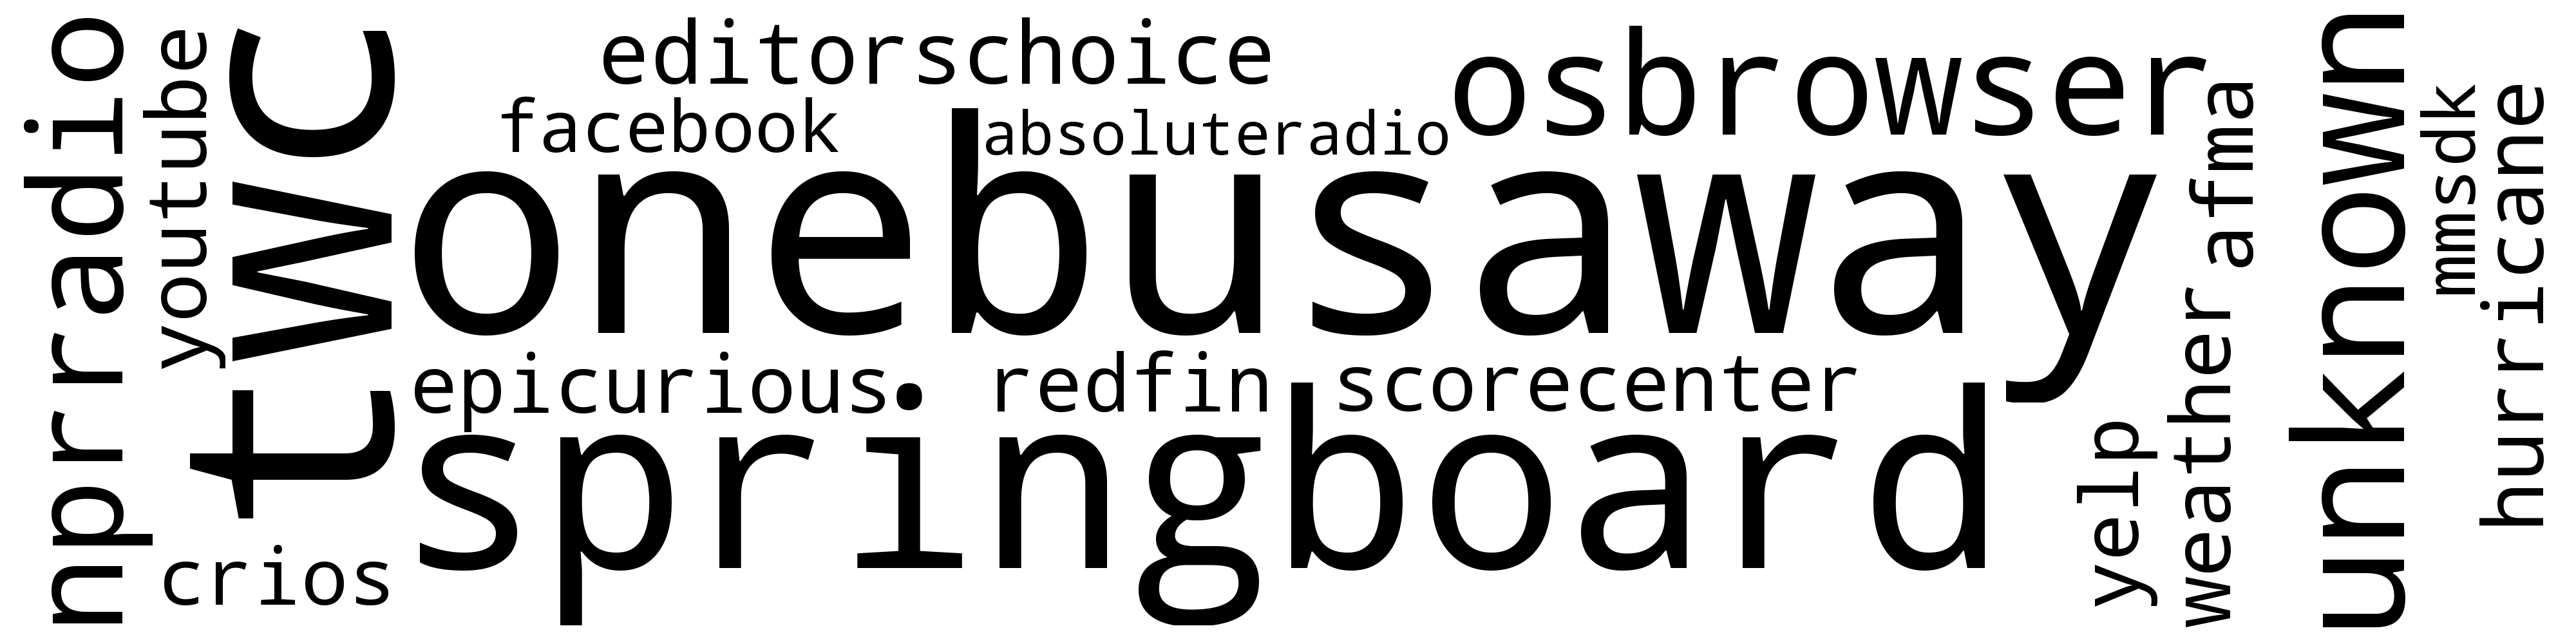
\includegraphics[width=\columnwidth]{figures/wordcloud_useragentsignature_location_image.png}
\newline
%\subfloat[Springboard \useragent strings leaking the device location.]{\label{fig:springboard}
%\begin{tabular}{|l|}
% \hline
% SpringBoard/50 CFNetwork/548.1.4 Darwin/11.0.0 \tabularnewline
% SpringBoard/50 CFNetwork/609 Darwin/13.0.0 \tabularnewline   
% SpringBoard/50 CFNetwork/609.1.4 Darwin/13.0.0 \tabularnewline
% \hline
% \end{tabular}}\newline
\subfloat[Frequency of leaks by \emph{SpringBoard}.]{\label{fig:springboard-wild} 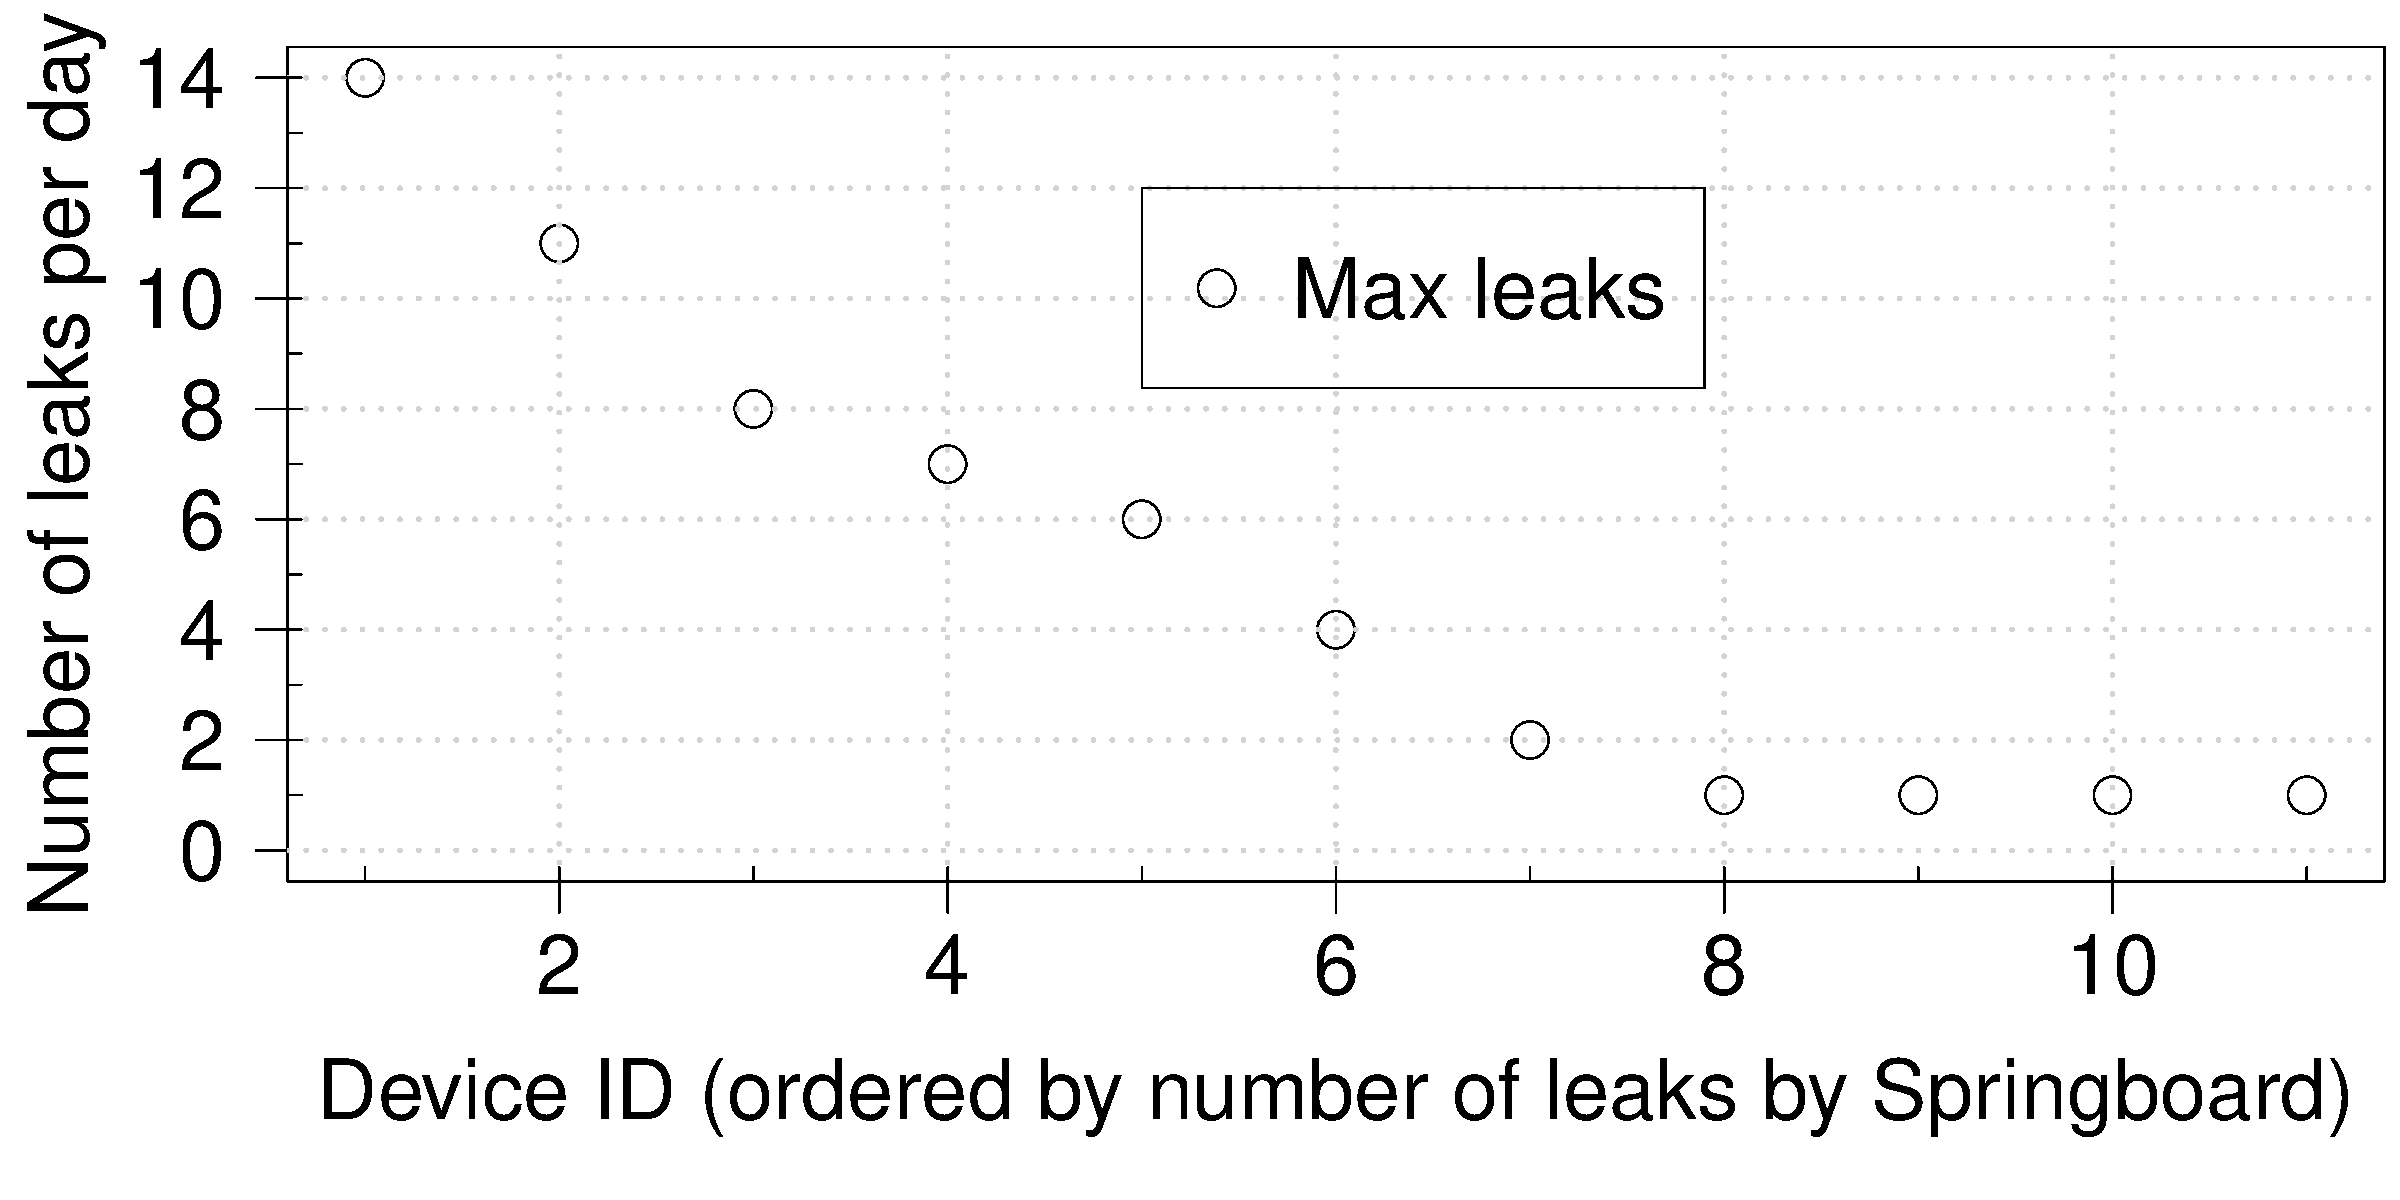
\includegraphics[width=0.9\columnwidth]{plots/piileaks_locclearspringboard.pdf}}
\caption{Apps that send the location information in the clear. \emph{The font size in the cloud represent the number of flows that sent the location information in the clear. We observe location leaks across different version of SpringBoard and from all the iPhones and the iPodtouch devices in the \mobWild dataset. }}
\label{fig:location-wordcloud}
\vspace{\postfigspace}
\end{figure}

In Figure~\ref{fig:location-wordcloud}, we present a \emph{word cloud} of
the apps that send the location information of the devices.
We observe that a bus service app (\emph{One Bus Away}), the
app that manages the iOS homescreen (\emph{SpringBoard}), and
weather apps (\emph{TWC}, \emph{Weather}, and \emph{Hurricane})
were responsible for more 78\% of the flows that sent the location
information in the clear. 
Further, \emph{SpringBoard} (the app responsible for managing the home screen of iOS devices) sends location information in the clear to fetch weather information from Yahoo servers. 
In Figure~\ref{fig:springboard-wild}, we observe that \emph{SpringBoard} leaked location information for 11 devices in the \mobWild dataset, a maximum of 14 leaks per day was observed for one device. 
We also observe that these devices include the iPodtouch device and all the iPhones in \mobWild, however, we do not observe such leaks for the iPad devices in the \mobWild dataset.  


In addition, we observe that the device ID and IMEI number of
devices in the \mobWild dataset are leaked in the clear.  Based on our
classification methodology, we observe that the IMEI number and device
ID is leaked by Web browsers; we do not observe any other app 
signature in non-browser flows leaking these IDs in the \mobWild dataset.  As in the case of
controlled experiments, A\&A sites are the most popular
destination for the IMEI number leaks.  Among the 16 sites that received 
the IMEI number in the clear, 10 are A\&A sites;
the rest of the sites includes sites for games, news, and manufacturer
updates.

\begin{table}
\centering
\begin{small}
\begin{tabular}{|p{0.35\columnwidth}|p{0.1\columnwidth}|p{0.15\columnwidth}|p{0.1\columnwidth}|}
\hline
\multirow{2}{*}{\bf Tracker} & \multicolumn{3}{c|}{\bf Number of devices tracked}\tabularnewline
\cline{2-4}
                      &  {\bf Total} & {\bf iOS} & {\bf Android} \tabularnewline
\hline
doubleclick.net       & 26 {\em(all)} & 15 {\em(all)} & 11 {\em(all)} \tabularnewline
\hline
google-analytics.com  & 26 {\em(all)} & 15 {\em(all)}  & 11 {\em(all)} \tabularnewline
\hline
googlesyndication.com & 22 & 12 & 10 \tabularnewline
\hline
admob.com             & 21 & 11 & 10 \tabularnewline
\hline
scorecardresearch.com &  21 & 11 & 10 \tabularnewline
\hline
\end{tabular}
\end{small}
\caption{The top 5 ads and analytics sites that were contacted by the devices in our dataset.
\emph{The sites, doubleclick.net and google-analytics.com, were contacted by all the 26 devices in} \mobWild.}
\label{tab:top-trackers}
\end{table}

In Table~\ref{tab:top-trackers}, we present the number of devices in the \mobWild dataset that contact the most popular A\&A sites, an activity that is receiving considerable attention~\cite{roesner:webtrackers,leontiadis:mobileads,vallina-rod:ads}.
We observe that all the devices in the \mobWild dataset contacted doubleclick.com, an ad site, and google-analytics.com, a tracking site. 
Further, 66.12\% of the ads and analytics traffic volume in the \mobWild dataset was from browsers, 6.46\% of the
traffic contained a blank user-agent field, and 4.8\% of the traffic contained a signature of \emph{Google-Analytics} library.
The rest of the traffic contained signatures of other apps such as Facebook, Pandora, and YouTube.

Given the extensive nature of tracking over mobile devices, we developed a tool, \emph{ConVis} that allows users to visualize their devices' tracking, and the apps that facilitate this tracking, with the help of a web-based interfaces similar to that of Mozilla Collusion~\cite{collusion}. \emph{ConVis} provides a visual interface that allows 
 users to specify block lists for connections based on (app, 3rd party) tuples. A demo of our tool is 
 located at \url{http://goo.gl/A17h9}. 
%\tbd{A demo of this can be found at ...}
%\tbd{Add some comment about ConVis (Nick's work), say that it's another 
%contribution in that it helps average users visualize their tracking and PII, 
%and that we make it available to participating users, and the URL for the 
%demo is at location X.}



%%% Local Variables: 
%%% mode: latex
%%% TeX-master: "main"
%%% End: 

%       getjar.com     & - S & - S \tabularnewline
%       aarki.net      & - S & - - \tabularnewline
%       chartboost.com & - S & - S \tabularnewline
%       *pocketexchange&   S &   S \tabularnewline
%       *vserv.mobi    & - - & C   \tabularnewline
%       *groupon.com   &     &   S
%       *flurry.com    &     &   S
%       *bankofamerica &     &   S
%       *google.com    & - - & - S

%\section{MISC}

% \begin{figure}
% \centering
% \includegraphics[width=\columnwidth]{plots/ads_wild_gatracking.pdf}
% \caption{Number of devices tracked by Google-Analytics. \emph{We observe that devices }}
% \label{fig:tracking-analytics}
% \end{figure}

% \begin{figure}
% \centering
% \includegraphics[width=\columnwidth]{plots/ads_wild_usertracking.pdf}
% \caption{Number of sites that track a user. \emph{We observe that devices }}
% \label{fig:tracking-analytics}
% \end{figure}

% \begin{figure}
% \centering
% \includegraphics[width=\columnwidth]{plots/ads_wild_sitescontacted.pdf}
% \caption{Number of visits to A\&A sites per device. \emph{The error bars indicate the 25$^{th}$ and 75$^{th}$ percentiles. Each visit is a potential tracking visit.}}
% \label{fig:tracking-analytics}
% \end{figure}

% \begin{table}    
%     \centering
%     \begin{small}
%     \begin{tabular}{|l|c|c|}
%        \hline
%        {\bf Host}&{\bf IMEI}&{\bf Device ID}\tabularnewline
%        \hline              
%        tapjoyads.com  & Y & - \tabularnewline
%        zynga.com      & Y & - \tabularnewline
%        iheart.com     & Y & Y \tabularnewline
%        google.com     & - & Y \tabularnewline
%        flurry.com     & - & Y \tabularnewline
%        \hline
%     \end{tabular}
%     \end{small}
%     \caption{Hosts to which the IMEI or Device ID was sent in the clear and over HTTPS. \emph{The value Y for a column implies that data was sent over HTTP and HTTPS. We order these hosts based on the number of flows that sent the IMEI number in the clear and over HTTPS.}}
%     \label{tab:pii-leakage-sites}
% \end{table}

%Moreover, we observe that 4\% of the flows
%sent the location information to ads and analytics sites; the rest of the
%flows being from apps including browsers, the Facebook app, and angry birds. 
% more than
%80\% of \emph{ad-flows} leaking location information did not include
%an application signature in the user-agent field, 
%Similarly, from the device of one of the authors of the paper, we observed that the latest three versions YahooMail application, up to the time of the measurements, leaked the user's email address in the clear.


%\tbd{This should come before 
%We first identify A\&A flows using the publicly available database of~\cite{YoyoAds}; we augment this list of domains using recent research on mobile ads~\cite{hornyack:appfence, leontiadis:mobileads}.
%Based on this classification, we observe that the ads and analytics traffic was responsible for up to 6\% of the traffic by volume per device, an observation in line to the one made by Vallina-Rodriguez~\etal~\cite{vallina-rod:ads}}.

%\subsection{Ads and Analytics in the Wild}

% \tbd{focusing on ads and analytics is just what you did in the
%   previous paragraph. What is new or different in this one.}
% We now focus our attention on the extent to which devices in the
% \mobWild dataset contact ads and analytics (A\&A) sites, an activity
% that is receiving considerable
% attention~\cite{roesner:webtrackers,leontiadis:mobileads,vallina-rod:ads}.
% Using our classification based on the \httphost, we observe that the
% ads and analytics traffic was responsible for up to 6\% of the traffic
% by volume per device, an observation in line with the one made by
% Vallina-Rodriguez~\etal~\cite{vallina-rod:ads}.  Rather that focusing
% on the traffic volume we focus on the extent to which these sites are
% able to track the users in the dataset and the applications that
% facilitate this tracking.
%\tbd{This must come before Furthermore, we observed that 7\% of the traffic contained the Google-Analytics in the signature field; this signature was observed even in the flows for users that did not have the Google Analytics application installed on the device. Mention that we will wrongly classify the flows from Google Analytics app as ads and analytics traffic} 

